\tikzset{
	%%% SPRING STYLING
 	set spring/.code={\pgfqkeys{/tikz/spring}{#1}},
 	set spring={length/.initial=6, amplitude/.initial=2mm},
	spring/.style={thick,decorate,decoration={aspect=0.5, segment length=\pgfkeysvalueof{/tikz/spring/length}, amplitude=\pgfkeysvalueof{/tikz/spring/amplitude},coil}},
 	%%% MASS STYLING
	mass/.style={ fill=red }
}

\section{Transition from a discrete to continuous system}
\label{sec:trans-from-discr}

Consider an infinite chain of equal mass particles spaced $a$ apart,
and connected by uniform, massless springs of force constant $k$,
illustrated in figure \ref{fig:springs}.

\begin{figure}[b]
  \centering
  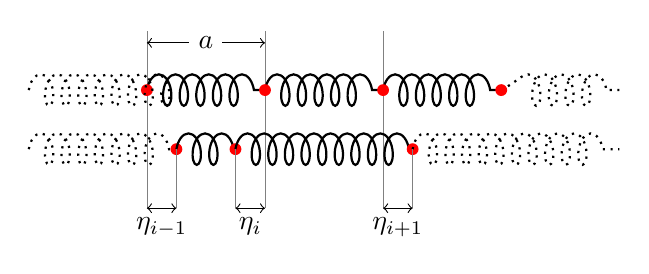
\begin{tikzpicture}[scale=0.75]
	\foreach \x in {2,4,...,6}{
		\draw [help lines]  (\x, -2) -- (\x, 1);
		\draw[spring={length=6}] (\x,0) -- (\x+2,0);
		\fill [mass] (\x,0) circle (0.1);
	}   \draw [dotted, spring] (0,0) -- (2,0) (8,0) -- (10,0);
	    \fill [mass] (8,0) circle (0.1);
	    \draw [<->] (2,0.8) -- (4,0.8) node [midway, fill=white] {$a$};

	                                   \draw[dotted, spring={length=2}] (0,-1) -- (2.5,-1);
	\fill [mass] (2.5, -1) circle (0.1); \draw[spring={length=2}] (2.5,-1) -- (3.5,-1);
	\fill [mass] (3.5, -1) circle (0.1); \draw[spring={length=2}] (3.5,-1) -- (6.5,-1);
	\fill [mass] (6.5, -1) circle (0.1); \draw[dotted, spring={length=2}] (6.5,-1) -- (10,-1);

	\draw [help lines] (2.5, -1) -- (2.5, -2); 
	\draw [<->] (2, -2) -- (2.5, -2) node [below, midway] {$\eta_{i-1}$};
	\draw [help lines] (3.5, -1) -- (3.5, -2);
	\draw [<->] (3.5, -2) -- (4, -2) node [below, midway] {$\eta_{i}$};
	\draw [help lines] (6.5, -1) -- (6.5, -2);
	\draw [<->] (6.5, -2) -- (6, -2) node [below, midway] {$\eta_{i+1}$};
\end{tikzpicture}
  \caption{A system of connected masses in a one-dimensional infinite system.}
  \label{fig:springs}
\end{figure}

The kinetic energy in the chain is given by
\begin{subequations}
  \begin{equation}
    \label{eq:61}
    T = \half \sum_i m_i \dot{\eta_i}^2
  \end{equation}
  where $\eta_i$ is the displacement of the $i$th particle from its
  equilibrium position. The potential energy from the springs is
  \begin{equation}
    \label{eq:62}
    V = \half \sum_i k (\eta_{i+1} - \eta_i)^2
  \end{equation}
\end{subequations}
The Lagrangian for the system is then
\begin{align}
  L & = T - V                                                                                          \nonumber\\
    & = \half \sum \qty( m \dot{\eta}^2 - k (\eta_{i+1} + \eta_i)^2 )                                  \nonumber\\
    & = \half \sum_i a \qty[ \frac{m}{a} \dot{\eta}_i^2 - k a \qty( \frac{\eta_{i+1} - \eta_i}{a} )^2] \nonumber\\
    & = \sum_i a L_i
\end{align}
where $a$ is the equilibrium separation of the masses. Thus
\begin{equation}
  \label{eq:63}
  \frac{m}{a} \ddot{\eta}_i - ka \qty( \frac{\eta_{i+1} - \eta_i}{a^2} ) + ka \qty( \frac{\eta_i - \eta_{i-1}}{a^2} ) = 0
\end{equation}
As $a \to 0$ then $\frac{m}{a} \to \mu$, for $\mu$ the linear mass
density. Then, from Hooke's Law
\begin{equation}
  \label{eq:64}
  F = Y \xi = k( \eta_{i+1} - \eta_i ) = k a \xi
\end{equation}
for $Y$ the Young's modulus, and $\xi$ the relative extension,
\[ \xi = \frac{\eta_{i+1} - \eta_i}{a} \] Then, in the continuous
limit $x_i$ becomes a coordinate, so $x_i \to x$, so
\[ \frac{\eta_{i+1} - \eta_i}{a} \to \frac{\eta(x+a) - \eta(x)}{a} \to \dv{\eta}{x} \]
as $a \to 0$. Thus
\begin{equation}
  \label{eq:65}
  L = \half \int \qty[ \mu \dot{\eta}^2 - Y \qty( \dv{\eta}{x} )^2] \dd{x}
\end{equation}
and as $a \to 0$,
\[ 
\lim_{a \to 0} \qty( - \frac{Y}{a} \qty[ \eval{\dv{\eta}{x}}_x - \eval{ \dv{\eta}{x}  }_{x-a} ] ) \to \dv[2]{\eta}{x} Y
\]
Thus
\begin{equation}
  \label{eq:66}
  \mu \dv[2]{\eta}{t} - Y \dv{\eta}{x} = 0 \iff \mathcal{L} = \half \qty[\mu \qty(\dv{\eta}{t})^2 - Y \qty(\dv{\eta}{x})^2]
\end{equation}
Where $\mathcal{L}$ is the Lagrangian density. For an elastic rod, the
$\mathcal{L}$ has an $\dv{\eta}{t}$ and $\dv{\eta}{x}$ term, so
$\vec{x}$ and $t$ can have similar roles. If a local force was present
there would be a dependence on $\eta$ and $\nabla \eta$, so a general
form for $\mathcal{L}$ is
\begin{equation}
  \label{eq:67}
  \mathcal{L} = \mathcal{L}\qty(\eta, \dv{\eta}{x}, \dv{\eta}{t}, x, t) 
\end{equation}

\section{The principle of least action for fields}
\label{sec:princ-least-acti}

The principle of least action is now
\begin{equation}
  \label{eq:68}
  \delta I = \delta \int_1^2 \int \mathcal{L} \dd{x} \dd{t} = 0
\end{equation}

Noting that $x$ and $t$ are unaffected by variations, as they have
fixed end points, then the variation in $\eta$ is
\begin{equation}
  \label{eq:69}
  \eta(x,t; \alpha) = \eta(x, t; 0) + \alpha \zeta(x,t)
\end{equation}
Where $\eta(x,t;0)$ is the correct solution, and $\zeta(x,t)$
disappears at $x_1, x_2, t_1, t_2$. Also, for $I$ to be a function of
$\alpha$, and to be an extremum of $\eta(x,t,;0)$ its derivative with
respect to $\alpha$ must vanish at $\alpha=0$.

\begin{align}
  \label{eq:70}
  \dv{I}{\alpha} = \int_{t_1}^{t_{2}} \int_{x_1}^{x_2} \dd{x} & \dd{t} \bigg[ \pdv{\mathcal{L}}{\eta} \pdv{\eta}{\alpha} + \pdv{\mathcal{L}}{\pdv{\eta}{t}} \pdv{\alpha} \qty(\dv{\eta}{t}) + \nonumber\\
& \qquad \pdv{\mathcal{L}}{\pdv{\eta}{x}} \pdv{\alpha} \qty( \dv{\eta}{x} ) \bigg]
\end{align}
We know $a \zeta$ disappears at the end-points, so
\begin{subequations}
  \begin{align}
    \int_{t_1}^{t_2} \pdv{\mathcal{L}}{\pdv{\eta}{t}} \pdv{\alpha} \qty( \dv{\eta}{t} ) \dd{t} &= - \int_{t_1}^{t_2} \dv{t} \qty( \pdv{\mathcal{L}}{\pdv{\eta}{t}} ) \pdv{\eta}{\alpha} \dd{t} \\
\int_{x_1}^{x_2} \pdv{\mathcal{L}}{\pdv{\eta}{x}} \pdv{\alpha} \qty( \dv{\eta}{x} ) \dd{x} &= - \int_{x_1}^{x_2} \dv{x} \qty( \pdv{\mathcal{L}}{\pdv{\eta}{x}} ) \pdv{\eta}{\alpha} \dd{x} 
  \end{align}
Thus
\[ \iint \qty[ \pdv{\mathcal{L}}{\eta} - \dv{t} \qty( \pdv{\mathcal{L}}{\pdv{\eta}{t}} ) - \dv{x} \qty( \pdv{\mathcal{L}}{\pdv{\eta}{x}} ) ] \eval{\pdv{\eta}{\alpha}}_0 = 0 \]
\end{subequations}
So,
\begin{equation}
  \label{eq:71}
  \dv{t} \pdv{\mathcal{L}}{\dot{\eta}} + \dv{x} \pdv{\mathcal{L}}{\eta'} - \pdv{\mathcal{L}}{\eta} = 0
\end{equation}
are the Euler-lagrange equations for a continuous system. Note that
equation \eqref{eq:71} has the form of a single equation, but since
$\eta$ is a differential equation it provides the many solutions to
make the combination an infinite system. Adopting the comma notation
for field derivatives,
\begin{equation}
  \label{eq:72}
  \mathcal{L} = \mathcal{L}(\eta_{\rho}, \eta_{\rho, \nu} x^{\nu}), \qquad L = \int \mathcal{L} (\dd{x^i})
\end{equation}
and the principle of least action has the form
\[ \delta I = \delta \int \mathcal{L}(\dd{x^{\mu}}) = 0 \]
thus
\begin{equation}
  \label{eq:73}
  \dv{x^{\nu}} \qty[ \pdv{\mathcal{L}}{\eta_{\rho, \nu}}] - \pdv{\mathcal{L}}{\eta_{\rho}} = 0
\end{equation}
are the General Euler-Lagrange equations for the 4-vector field.

\section{The stress-energy tensor}
\label{sec:stress-energy-tensor}

An analogue to the energy function then exists,
\begin{align*}
  \pdv{\mathcal{L}}{x^{\mu}} &= \pdv{\mathcal{L}}{\eta_{\rho}} \eta_{\rho,\mu} + \pdv{\mathcal{L}}{\eta_{\rho, \nu}} \eta_{\rho, \mu\nu}+\pdv{\mathcal{L}}{x^{\mu}} \\
&= \dv{x^{\nu}} \qty[\pdv{\mathcal{L}}{\eta_{\rho,\nu}}] \eta_{\rho,\mu} + \pdv{\mathcal{L}}{\eta_{\rho,\nu}} \dv{\eta_{\rho,\mu}}{x^{\nu}} + \pdv{\mathcal{L}}{x^{\mu}} + \pdv{\mathcal{L}}{x^{\mu}} \\ &\qquad\text{(using the Euler-Lagrange equation)} \\
&= \dv{x^{\nu}} \qty[ \pdv{\mathcal{L}}{\eta_{\rho,\nu}} \eta_{\rho,\mu}] + \pdv{\mathcal{L}}{x^{\mu}} \\
- \pdv{\mathcal{L}}{x^{\mu}} &= \dv{x^{\nu}} \qty[ \pdv{\mathcal{L}}{\eta_{\rho, \nu}} \eta_{\rho,\mu} - \mathcal{L} \delta_{\mu \nu}] \tag{\(\star\)}
\end{align*}
Suppose the field doesn't depend upon $x^{\mu}$; a free-field (with no
driving forces or sinkes at explicit points, so doesn't interact with
particles) then ($\star$) has the form of divergence equations,
\[ \tensor{T}{_{\mu}^{\nu}_{,\nu}} = 0 \]
where
\begin{equation}
  \label{eq:74}
  \tensor{T}{_{\mu}^{\nu}} = \pdv{\mathcal{L}}{\eta_{\rho, \nu}} \eta_{\rho, \mu} - \mathcal{L} \delta_{\mu}^{\nu}
\end{equation}
is the stress-energy tensor.

The components represent a number of important quantities,

\begin{centering}
    \begin{tikzpicture}
        \matrix [matrix of math nodes,left delimiter=(,right delimiter=)] (m)
        {
            T^{00} & T^{01} & T^{02} & T^{03} \\
            T^{10} & T^{11} & T^{12} & T^{13} \\
            T^{20} & T^{21} & T^{22} & T^{23} \\
            T^{30} & T^{31} & T^{32} & T^{33} \\
        };  
        \fill[opacity=0.2, color=accent-blue] 
             (m-1-1.north west) -- (m-1-1.north east) -- (m-1-1.south east) -- (m-1-1.south west) -- (m-1-1.north west);
        \fill[opacity=0.2,color=accent-red] 
             (m-1-2.north west) -- (m-1-4.north east) -- (m-1-4.south east) -- (m-1-2.south west) -- (m-1-2.north west);
        \fill[opacity=0.2,color=accent-red] 
             (m-2-1.north west) -- (m-2-1.north east) -- (m-4-1.south east) -- (m-4-1.south west) -- (m-2-1.north west);
        \fill[opacity=0.2,color=accent-yellow] 
             (m-2-2.north west) -- (m-4-2.south west) -- (m-4-4.south east) -- (m-3-2.north east);
\fill[opacity=0.2, color=accent-purple]
(m-2-4.north east) -- (m-4-4.south east) -- (m-2-2.north west) -- (m-2-4.north east);
        \fill[opacity=0.2, color=accent-green] 
             (m-2-2.north west) -- (m-2-2.south west) -- (m-4-4.south west) -- (m-4-4.south east)
          -- (m-4-4.north east) -- (m-2-2.north east) -- cycle;
      \end{tikzpicture}

These are 
{ \color{accent-blue} energy density },
{ \color{accent-red} momentum density},
{ \color{accent-yellow} momentum flux},
{\color{accent-green} pressure}, and
{\color{accent-purple} shear stress}.
    \end{centering}
    
%%% Local Variables: 
%%% mode: latex
%%% TeX-master: "../project"
%%% End: 
